%Préambule du document :
\documentclass[12pt, a4paper]{book}
%\usepackage[latin1]{inputenc} 
\usepackage[utf8]{inputenc} % accents
\usepackage{gensymb} % degree symbol ° (\degree)
\usepackage[T1]{fontenc} % | "`pipe"' character
\usepackage{graphicx}
\usepackage{titling}
\usepackage{amssymb} 
\usepackage{minitoc} % chapter's tocs
\usepackage{authblk} % author affiliations
\usepackage{fancyhdr} % modify the headers
\usepackage{tabularx} % tables not larger than A4
\usepackage[table]{xcolor} %colors inside the tables
\usepackage{float}
\usepackage{multicol} % multiple columns in some sections
\usepackage[inner=2cm,outer=2cm]{geometry} %A4 margins
\usepackage{siunitx}
\usepackage[labelfont=bf, margin=0.5cm]{caption} % for figure captions in minipages
\usepackage{hyperref} %link references (toc, citations) inside document
\usepackage{natbib} % to cite with parentheses and plain text et only year if you please...
\usepackage{amsmath}
 \usepackage{fixltx2e} % allows overrightarrow to be in caption

\hyphenation{Cur-vature} %Example of hyphenation

 \MakeRobust{\overrightarrow}


\bibliographystyle{plainnat} % reference style
\renewcommand{\bibname}{References} %Rename "`bibliography"' => "`references"'
\newcommand*{\doi}[1]{\href{https://doi.org/#1}{doi: #1}}


\hypersetup{
    colorlinks,
    citecolor=brown,
    filecolor=green,
    linkcolor=red,
    urlcolor=blue
}
\hypersetup{linktocpage}


\pagestyle{fancy}
\fancyhead{}
\fancyfoot{}
\fancyhead[RO,LE]{\thepage}
\fancyhead[LO]{\leftmark}
\fancyhead[RE]{\rightmark}
\setcounter{tocdepth}{1} % we only want chapters and sections in toc
\setcounter{minitocdepth}{2} %we want sections and subsections in chapters' minitocs

\pretitle{%
  \begin{center}
  
  
\includegraphics[width=17cm]{../Logo_software.png}\\[\bigskipamount]
}
\posttitle{
\\
  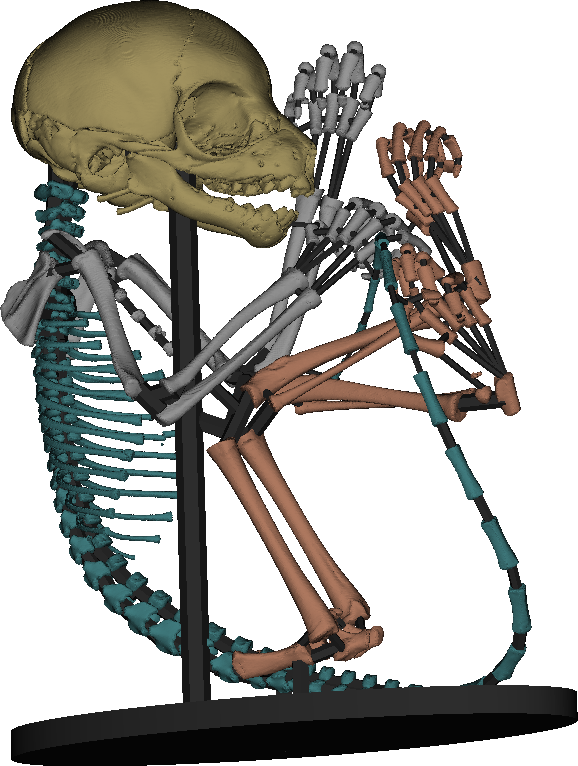
\includegraphics[width=8cm]{tutorial10.png}\\[\bigskipamount]
\end{center}}

%\postdate{
%
\includegraphics[width=15cm]{logo_affiliations.png}
%}

\title{Tutorial 10: 3D printing using connective struts}



%\titlepicture[width=13cm]{Logo_software.png}
\author{Renaud LEBRUN}
\affil{Institut des Sciences de l'Evolution, Université de Montpellier, France}
\date{\today} 

\def\chaptername{Tutorial}
\setcounter{chapter}{10}
%Corps du document :
\begin{document}

	\dominitoc

\maketitle


\faketableofcontents

%\chapter{Working with landmarks}
\addstarredchapter{3D printing using connective struts}

\markboth{Tutorial 10: 3D printing using connective struts}{}

\minitoc 
Tutorial 10 includes:
\begin{itemize}
\item One .ntw (MorphoDig project) file
\item Four .vtk surface +.pos files representing the skeleton (skull, vertebrae+ribs, upper limbs and lower limbs) of a newborn \textit{Lemur catta}.
\item 222 .vtk surface + .pos files representing cylindric connective struts.
\item The present .pdf document
\end{itemize}



\section{About the specimen}
The 3D model corresponds to a virtually reconstructed skeleton of a newborn \textit{Lemur catta} from the Université de Montpellier (inventory number: UM-ISEM-805V). This specimen was born in captivity in the Zoo de Lunaret, Montpellier, France. The 3D data were obtained by computerized microtomography at the MRI \si{\micro}CT platform housed at the ISEM. 

\section{About the 3D data}
Resolution, Amira.
\section{A brief overview of enclosed files}
		
The present tutorial contains a project .ntw file, which is useful to open the whole project with all the connective struts in a convenient position. Open the enclosed .ntw file (File->Open Project, then select "Lemur\_catta\_805V.ntw"). 


\section{Tutorial}

\subsection{Connective struts}
Connective struts are created by clicking on .\\ 


\begin{figure}
  \centering
  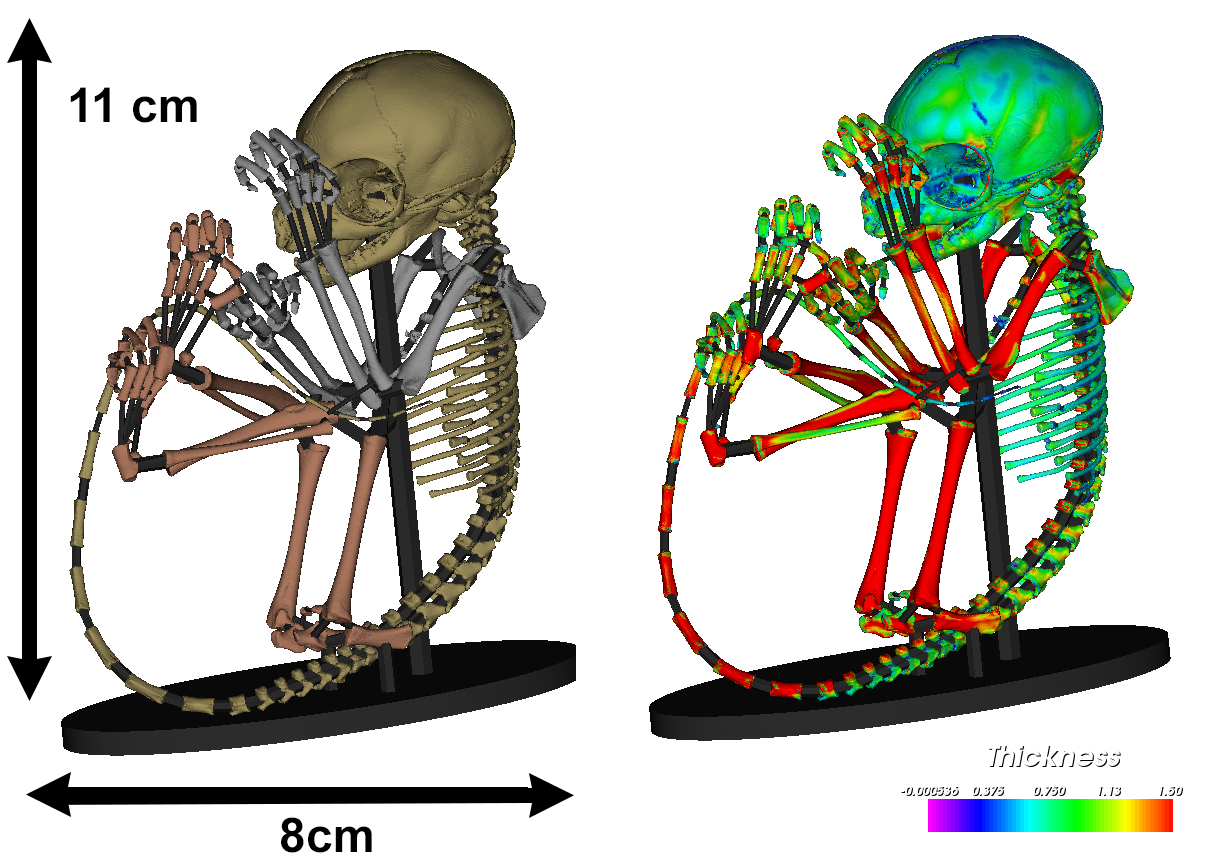
\includegraphics[scale=0.5]{lemur_catta.png} 
	\caption{lemur catta.}
\label{lemur_catta}
\end{figure}

\subsection{Export as .stl}


\section{Acknowledgements}
Thanks to the MRI platform for MicroCT data acquisition. T


%\nocite{*}   % All bibliography items appear without citation in the text

%\cleardoublepage
%\phantomsection

%\addcontentsline{toc}{section}{References}
%\bibliography{References}	

\end{document} 

